%\documentclass[a4paper,11pt]{book}
\documentclass[a4paper,twoside,11pt,titlepage]{book}
\usepackage{listings}
\usepackage[utf8]{inputenc}
\usepackage[spanish]{babel}

\usepackage[utf8]{inputenc}
\usepackage[spanish,es-tabla]{babel}
\usepackage{graphicx}
\usepackage{subcaption}
\usepackage[dvips]{epsfig}
\usepackage{amssymb}
\usepackage{eurosym}
\usepackage{float}
\usepackage{latexsym}
\usepackage{a4}
\usepackage{listings}
\usepackage[hidelinks]{hyperref} 
\usepackage{multirow} % para las tablas
\usepackage{tabularx}

\newcolumntype{C}[1]{>{\centering\arraybackslash}p{#1}} %para determinar ancho de columna centrada
\newcolumntype{L}[1]{>{\arraybackslash}p{#1}} %para determinar ancho de columna de columna a la izquierda

% \usepackage[style=list, number=none]{glossary} %
%\usepackage{titlesec}
%\usepackage{pailatino}

\decimalpoint
\usepackage{dcolumn}
\newcolumntype{.}{D{.}{\esperiod}{-1}}
\makeatletter
\addto\shorthandsspanish{\let\esperiod\es@period@code}
\makeatother


%\usepackage[chapter]{algorithm}
\RequirePackage{verbatim}
%\RequirePackage[Glenn]{fncychap}
\usepackage{fancyhdr}
\usepackage{graphicx}
\usepackage{afterpage}

\usepackage{longtable}

\usepackage[pdfborder={000}]{hyperref} %referencia

% ********************************************************************
% Re-usable information
% ********************************************************************
\newcommand{\myTitle}{Título del proyecto :-)\xspace}
\newcommand{\myDegree}{Grado en ...\xspace}
\newcommand{\myName}{Guillermo Muriel Sánchez lafuente\xspace}
\newcommand{\myProf}{Nombre Apllido1 Apellido2 (tutor1)\xspace}
\newcommand{\myOtherProf}{Nombre Apllido1 Apellido2 (tutor2)\xspace}
%\newcommand{\mySupervisor}{Put name here\xspace}
\newcommand{\myFaculty}{Escuela Técnica Superior de Ingenierías Informática y de
Telecomunicación\xspace}
\newcommand{\myFacultyShort}{E.T.S. de Ingenierías Informática y de
Telecomunicación\xspace}
\newcommand{\myDepartment}{Departamento de ...\xspace}
\newcommand{\myUni}{\protect{Universidad de Granada}\xspace}
\newcommand{\myLocation}{Granada\xspace}
\newcommand{\myTime}{\today\xspace}
\newcommand{\myVersion}{Version 0.1\xspace}


\hypersetup{
pdfauthor = {\myName (email (en) ugr (punto) es)},
pdftitle = {\myTitle},
pdfsubject = {},
pdfkeywords = {palabra_clave1, palabra_clave2, palabra_clave3, ...},
pdfcreator = {LaTeX con el paquete ....},
pdfproducer = {pdflatex}
}

%\hyphenation{}


%\usepackage{doxygen/doxygen}
%\usepackage{pdfpages}
\usepackage{url}
\usepackage{colortbl,longtable}
\usepackage[stable]{footmisc}
%\usepackage{index}

%\makeindex
%\usepackage[style=long, cols=2,border=plain,toc=true,number=none]{glossary}
% \makeglossary

% Definición de comandos que me son tiles:
%\renewcommand{\indexname}{Índice alfabético}
%\renewcommand{\glossaryname}{Glosario}

\pagestyle{fancy}
\fancyhf{}
\fancyhead[LO]{\leftmark}
\fancyhead[RE]{\rightmark}
\fancyhead[RO,LE]{\textbf{\thepage}}
\renewcommand{\chaptermark}[1]{\markboth{\textbf{#1}}{}}
\renewcommand{\sectionmark}[1]{\markright{\textbf{\thesection. #1}}}

\setlength{\headheight}{1.5\headheight}

\newcommand{\HRule}{\rule{\linewidth}{0.5mm}}
%Definimos los tipos teorema, ejemplo y definición podremos usar estos tipos
%simplemente poniendo \begin{teorema} \end{teorema} ...
\newtheorem{teorema}{Teorema}[chapter]
\newtheorem{ejemplo}{Ejemplo}[chapter]
\newtheorem{definicion}{Definición}[chapter]

\definecolor{gray97}{gray}{.97}
\definecolor{gray75}{gray}{.75}
\definecolor{gray45}{gray}{.45}
\definecolor{gray30}{gray}{.94}

\lstset{ frame=Ltb,
     framerule=0.5pt,
     aboveskip=0.5cm,
     framextopmargin=3pt,
     framexbottommargin=3pt,
     framexleftmargin=0.1cm,
     framesep=0pt,
     rulesep=.4pt,
     backgroundcolor=\color{gray97},
     rulesepcolor=\color{black},
     %
     stringstyle=\ttfamily,
     showstringspaces = false,
     basicstyle=\scriptsize\ttfamily,
     commentstyle=\color{gray45},
     keywordstyle=\bfseries,
     %
     numbers=left,
     numbersep=6pt,
     numberstyle=\tiny,
     numberfirstline = false,
     breaklines=true,
   }
 
% minimizar fragmentado de listados
\lstnewenvironment{listing}[1][]
   {\lstset{#1}\pagebreak[0]}{\pagebreak[0]}

\lstdefinestyle{CodigoC}
   {
	basicstyle=\scriptsize,
	frame=single,
	language=C,
	numbers=left
   }
\lstdefinestyle{CodigoC++}
   {
	basicstyle=\small,
	frame=single,
	backgroundcolor=\color{gray30},
	language=C++,
	numbers=left
   }

 
\lstdefinestyle{Consola}
   {basicstyle=\scriptsize\bf\ttfamily,
    backgroundcolor=\color{gray30},
    frame=single,
    numbers=none
   }


\newcommand{\bigrule}{\titlerule[0.5mm]}


%Para conseguir que en las páginas en blanco no ponga cabecerass
\makeatletter
\def\clearpage{%
  \ifvmode
    \ifnum \@dbltopnum =\m@ne
      \ifdim \pagetotal <\topskip
        \hbox{}
      \fi
    \fi
  \fi
  \newpage
  \thispagestyle{empty}
  \write\m@ne{}
  \vbox{}
  \penalty -\@Mi
}
\makeatother

\usepackage{pdfpages}
\begin{document}
\begin{titlepage}
 
 
\newlength{\centeroffset}
\setlength{\centeroffset}{-0.5\oddsidemargin}
\addtolength{\centeroffset}{0.5\evensidemargin}
\thispagestyle{empty}

\noindent\hspace*{\centeroffset}\begin{minipage}{\textwidth}

\centering

\includegraphics[width=0.9\textwidth]{imagenes/logo_ugr.jpg}\\[1.4cm]

\textsc{ \Large TRABAJO FIN DE GRADO\\[0.2cm]}
\textsc{ INGENIERÍA EN ...}\\[1cm]
% Upper part of the page
% 
% Title
{\Huge\bfseries Titulo del Proyecto\\
}
\noindent\rule[-1ex]{\textwidth}{3pt}\\[3.5ex]
{\large\bfseries Subtitulo del Proyecto}
\end{minipage}

\vspace{2.5cm}
\noindent\hspace*{\centeroffset}\begin{minipage}{\textwidth}
\centering

\textbf{Autor}\\ {\myName}\\[2.5ex]
\textbf{Directores}\\
{Nombre Apellido1 Apellido2 (tutor1)\\
Nombre Apellido1 Apellido2 (tutor2)}\\[2cm]

\includegraphics[width=0.3\textwidth]{imagenes/etsiit_logo.png}\\[0.1cm]
\textsc{Escuela Técnica Superior de Ingenierías Informática y de Telecomunicación}\\
\textsc{---}\\
Granada, mes de 201
\end{minipage}
%\addtolength{\textwidth}{\centeroffset}
%\vspace{\stretch{2}}
\end{titlepage}



\chapter*{}
%\thispagestyle{empty}
%\cleardoublepage

%\thispagestyle{empty}

\begin{titlepage}
 
 
\setlength{\centeroffset}{-0.5\oddsidemargin}
\addtolength{\centeroffset}{0.5\evensidemargin}
\thispagestyle{empty}

\noindent\hspace*{\centeroffset}\begin{minipage}{\textwidth}

\centering
%
\includegraphics[width=0.9\textwidth]{imagenes/logo_ugr.jpg}\\[1.4cm]

%\textsc{ \Large PROYECTO FIN DE CARRERA\\[0.2cm]}
%\textsc{ INGENIERÍA EN INFORMÁTICA}\\[1cm]
% Upper part of the page
% 

 \vspace{3.3cm}

%si el proyecto tiene logo poner aquí

\includegraphics{imagenes/logo_riddling.png} 
 \vspace{0.5cm}

% Title

{\Huge\bfseries \myTitle\\
}
\noindent\rule[-1ex]{\textwidth}{3pt}\\[3.5ex]
{\large\bfseries Una aplicación en la nube\\[4cm]}
\end{minipage}

\vspace{2.5cm}
\noindent\hspace*{\centeroffset}\begin{minipage}{\textwidth}
\centering

\textbf{Autor}\\ \myName\\[2.5ex]
\textbf{Directores}\\\myProf\\[2cm]
%
\includegraphics[width=0.15\textwidth]{imagenes/tstc.png}\\[0.1cm]
\textsc\myDepartment\\
%\textsc{---}\\
Granada, septiembre de 2018
\end{minipage}
%\addtolength{\textwidth}{\centeroffset}
\vspace{\stretch{2}}

 
\end{titlepage}






\cleardoublepage
\thispagestyle{empty}

\begin{center}
{\large\bfseries Título del Proyecto: Subtítulo del proyecto}\\
\end{center}
\begin{center}
Nombre Apellido1 Apellido2 (alumno)\\
\end{center}

%\vspace{0.7cm}
\noindent{\textbf{Palabras clave}: palabra\_clave1, palabra\_clave2, palabra\_clave3, ......}\\

\vspace{0.7cm}
\noindent{\textbf{Resumen}}\\

Poner aquí el resumen.
\cleardoublepage


\thispagestyle{empty}


\begin{center}
{\large\bfseries Project Title: Project Subtitle}\\
\end{center}
\begin{center}
First name, Family name (student)\\
\end{center}

%\vspace{0.7cm}
\noindent{\textbf{Keywords}: Keyword1, Keyword2, Keyword3, ....}\\

\vspace{0.7cm}
\noindent{\textbf{Abstract}}\\

Write here the abstract in English.

\chapter*{}
\thispagestyle{empty}

\noindent\rule[-1ex]{\textwidth}{2pt}\\[4.5ex]

Yo, \textbf{Nombre Apellido1 Apellido2}, alumno de la titulación TITULACIÓN de la \textbf{Escuela Técnica Superior
de Ingenierías Informática y de Telecomunicación de la Universidad de Granada}, con DNI XXXXXXXXX, autorizo la
ubicación de la siguiente copia de mi Trabajo Fin de Grado en la biblioteca del centro para que pueda ser
consultada por las personas que lo deseen.

\vspace{6cm}

\noindent Fdo: Nombre Apellido1 Apellido2

\vspace{2cm}

\begin{flushright}
Granada a X de mes de 201 .
\end{flushright}


\chapter*{}
\thispagestyle{empty}

\noindent\rule[-1ex]{\textwidth}{2pt}\\[4.5ex]

D. \textbf{Nombre Apellido1 Apellido2 (tutor1)}, Profesor del Área de XXXX del Departamento YYYY de la Universidad de Granada.

\vspace{0.5cm}

D. \textbf{Nombre Apellido1 Apellido2 (tutor2)}, Profesor del Área de XXXX del Departamento YYYY de la Universidad de Granada.


\vspace{0.5cm}

\textbf{Informan:}

\vspace{0.5cm}

Que el presente trabajo, titulado \textit{\textbf{Título del proyecto, Subtítulo del proyecto}},
ha sido realizado bajo su supervisión por \textbf{Nombre Apellido1 Apellido2 (alumno)}, y autorizamos la defensa de dicho trabajo ante el tribunal
que corresponda.

\vspace{0.5cm}

Y para que conste, expiden y firman el presente informe en Granada a X de mes de 201 .

\vspace{1cm}

\textbf{Los directores:}

\vspace{5cm}

\noindent \textbf{Nombre Apellido1 Apellido2 (tutor1) \ \ \ \ \ Nombre Apellido1 Apellido2 (tutor2)}

\chapter*{Agradecimientos}
\thispagestyle{empty}

       \vspace{1cm}


Poner aquí agradecimientos...


\frontmatter
\tableofcontents
\listoffigures
\listoftables

\mainmatter
\setlength{\parskip}{5pt}

\chapter{Introducción}
El ser humano es considerado un ser curioso, inquieto y siempre en busca de la aventura. No hay más que pararse a observar a un niño con un año de edad y comprobarlo.

Nuestra especie necesita retos a los que enfrentarse para crecer y mejorar. En definitiva, abrir la mente para evolucionar.

El mundo en el que vivimos nos plantea diariamente una serie de obstáculos que tenemos que superar día a día. Este trabajo, se realiza la mayor parte de las veces de una manera mecánica. Es decir, durante esa actividad, el cerebro no está usándose a pleno rendimiento. No estamos motivados.

Sin embargo, con la aparición de los juegos, al ser humano se le ofrece una actividad distinta, se le permite crujir su rutina.

Volviendo al origen de nuestra especie, nos adentramos en nuestra principal característica evolutiva, la resolución de problemas, tan fundamental para el desarrollo de nuestro intelecto.

He aquí la idea principal del proyecto, que no es otra que la de generar esa posibilidad que ayude al ser humano a su desarrollo. Todo esto apoyado mediante la creación de un juego conversacional. Gracias al cual se planteen y resuelvan acertijos de los más ingeniosos. 

Acertijos propuestos por individuos con alma de detective y resueltos por los mismos.

\section{Motivación y objetivo}

El poder colaborar en el desarrollo intelectual y en el entretenimiento de las personas es motivación más que suficiente para embarcarse en un proyecto de tal magnitud y dificultad.

Actualmente, cuando se decide crear un juego conversacional, se tienen al alcance de la mano, a través de internet, infinitas posibilidades para su creación.

El principal objetivo de este juego es que sea desarrollado con de una manera actual, teniendo muy en cuenta filosofías de desarrollo de software ágiles y con eje fundamental el software libre. 

Con el objeto adicional de que esté proyecto estará liberado bajo la licencia \textit{GNU General Public License v3.0} \cite{licenciaproyecto} y alojado en un repositorio público en GitHub.

Este juego deberá ser accesible desde cualquier plataforma, por lo que para ello será fundamental su desarrollo mediante un servicio en la nube, es decir, el paradigma del 'Cloud Computing' o 'Computación en la nube' \cite{nube1} estará muy presente en este proyecto.

\section{Descripción del proyecto}

El proyecto consistirá en el desarrollo de una aplicación cliente-servidor desplegada en la nube, adaptable a cualquier tipo de \textit{front-end} \cite{frontback} o interfaz.

Este proyecto tendrá especial énfasis en el servidor o \textit{back-end} \cite{frontback}, pero sin olvidar la parte de interfaz, ya que se busca que los usuarios se enganchen a este juego.

Para la parte de servidor, se desarrollará una \textit{API REST} \cite{api1} \cite{api2} \cite{api3}, que nos permitirá la comunicación desde la interfaz hasta los datos alojados en la nube, añadiendo la capa de abstracción necesaria para que la aplicación sea adaptable, en un futuro, a diferentes tipos de \textit{front-end} o interfaces. 

Esta aplicación se desarrollará mediante la filosofía o práctica \textit{DevOps} \cite{devops1} \cite{devops2} \cite{devops3} \cite{devops4}. En este proyecto será fundamental el desarrollo ágil de software y el monitoreo en todas las fases de su desarrollo, desde la integración hasta el despliegue e implementación.

Este proyecto se llamará \textit{Project X}, y estará alojado en la plataforma GitHub en un repositorio del mismo nombre que el proyecto \cite{proyectogithub}. Esta plataforma facilita enormemente el desarrollo ágil y la filosofía \textit{DevOps} nombrada anteriormente, haciendo que sea fácil el seguimiento de todas y cada una de las modificaciones realizadas en el proyecto y su continua integración y despliegue.

\section{Estructura de la memoria}

\begin{itemize}
    \item \textbf{Capítulo 1. Introducción}: el presente capítulo, es una breve introducción al trabajo realizado. 
    \item \textbf{Capítulo 2. Gestión y planificación del proyecto}: cómo se ha realizado la gestión del proyecto, metodología, planificación, riesgos y costes.
    \item \textbf{Capítulo 3. Especificación de requisitos}: descripción de los requisitos e historias de usuario del proyecto.
    \item \textbf{Capítulo 4. Análisis}: análisis de los requerimientos del sistema, tecnología y herramientas de desarrollo.
    \item \textbf{Capítulo 5. Diseño}: diseño de la aplicación, arquitectura y funcionamiento general.
    \item \textbf{Capítulo 6. Implementación}: implementación de los aspectos descritos en el capítulo de diseño anterior.
    \item \textbf{Capítulo 7. Pruebas}: verificación del software y validación del proyecto mediante tests unitarios.
    \item \textbf{Capítulo 8. Conclusiones y posibles ampliaciones}: conclusiones finales del proyecto, posibles ampliaciones y propuesta de mejoras.
\end{itemize}

\chapter{Gestión y Planificación del proyecto}
En este capítulo se tratarán todas las cuestiones relacionadas con la gestión del proyecto: la metodología de desarrollo escogida, la gestión del alcance, tiempo, riesgos y costes.

Lo que se busca con ello es determinar claramente los objetivos a cumplir durante la realización, así como asegurar el buen avance del proyecto repartiendo de forma adecuada los recursos, previniendo posibles problemas y estableciendo un marco de trabajo para estructurar, planificar y controlar el desarrollo del software.

\section{Gestión del alcance}
En esta sección se determinará el alcance general del proyecto, así como los criterios que serán necesarios para la aceptación de éste, y las restricciones a las que está sometido. Por último, se detallarán los entregables que se generarán al finalizar.

\subsection{Descripción del alcance del proyecto}
Para la creación de acertijos por parte de los usuarios y la posibilidad de que la comunidad de usuarios de la aplicación disponga de la posibilidad de poder resolver éstos e interactuar, es necesario tener en cuenta una serie de factores:

\begin{itemize}
    \item \textbf{Por parte de los usuarios:}
    \begin{itemize}
        \item \textbf{Datos personales del usuario:} será necesario almacenar datos personales tales como nombre y apellidos, contraseña y \textit{nick} o nombre de usuario.
        \item \textbf{Acertijos escritos:} es muy importante asociar cada usuario con el acertijo que él mismo ha escrito.
        \item \textbf{Propuestas de solución a acertijos:} también muy importante el registro en el sistema de las posibles propuestas de un usuario para la solución de los acertijos.
        \item \textbf{Valoración de las propuestas de solución a los acertijos del usuario:} un usuario podrá acceder a las soluciones propuestas para sus acertijos y puntuar según lo cerca que se encuentren de la solución final.
    \end{itemize}
    \item \textbf{Por parte de los acertijos:}
    \begin{itemize}
        \item \textbf{Datos específicos de cada acertijo:} será necesario almacenar el título, el acertijo, la solución al mismo, 3 pistas para facilitar el comienzo a los otros usuarios la búsqueda de la solución y el estado del porcentaje de resolución de la misma.
        \item \textbf{Acertijos escritos:} es muy importante asociar cada acertijo con el usuario que lo ha escrito.
        \item \textbf{Soluciones propuestas de cada acertijo:} también muy importante el registro en el sistema de las propuestas para la solución de cada acertijo.
    \end{itemize}
\end{itemize}

La aplicación contendrá dos funcionalidades principales, destacadas y que sustentarán el objetivo principal del proyecto: escritura de acertijos y resolución de los mismos.

Para la funcionalidad de escritura, el sistema será el encargado de almacenar los acertijos propuestos y mostrarlos al mundo. En la segunda funcionalidad nombrada, será el propio sistema el encargado de gestionar la interacción entre usuarios con el objetivo de resolver los enigmas.

\subsection{Criterios de aceptación}
El proyecto será aceptado si la aplicación será capaz de permitir a un usuario la escritura de un acertijo completo. Además, se podrá permitir al usuario proponer soluciones a distintos acertijos propuestos por otros usuarios. 

Por último, un usuario será capaz de poder evaluar las propuestas de solución de cada uno de sus acertijos y, éstos, automáticamente actualizarán su estado de resolución basándose en las puntuaciones de las mismas.
\subsection{Restricciones del proyecto}
El proyecto debe suponer un total de 12 créditos, es decir, unas 300 horas de trabajo, y debe ser entregado no más tarde del 07/09/2018.

\subsection{Entregables del proyecto}
Como resultado del proyecto se considerarán los siguientes entregables:
\begin{itemize}
    \item Código fuente de todo el software desarrollado.
    \item Memoria del trabajo de fin de grado.
\end{itemize}

\section{Metodología de desarrollo}
Antes de iniciar cualquier proyecto de desarrollo de software, es muy importante determinar y definir qué metodología se seguirá. El objetivo es establecer un plan de acción, reduciendo así el riesgo de que se sufran retrasos en el desarrollo, sobre costes, o un mal planteamiento que suponga el fracaso del proyecto en su totalidad. Probablemente en la práctica existan tantas metodologías de trabajo como proyectos de desarrollo, pero en todos los casos es necesario tener en cuenta las características y particularidades del proyecto a la hora de elegir y adaptar una metodología concreta al caso específico.

En el caso concreto de este proyecto, nos encontramos con varios factores importantes que resultan determinantes para la elección de una metodología concreta:

\begin{itemize}
    \item Al tratarse de una aplicación que necesita de interfaz, es necesario dedicar tiempo al desarrollo de la misma de una manera independiente a las demás partes. 
    \item En esta aplicación será necesaria la creación de una base de datos donde almacenar todos los acertijos, usuarios y propuestas de solución.
    \item Al tener que desarrollar una \textit{API Rest} que gestione las peticiones desde nuestra interfaz y nuestra base de datos, será necesario dedicar tiempo para el desarrollo de la misma, no de manera independiente, pues se necesita previamente una conexión de ésta con la base de datos.
\end{itemize}

Por ello, como metodología de desarrollo para mi proyecto lo mejor es crear una mezcla entre la metodología/framework  y la filosofía/práctiva \textit{DevOps}.

El lado \textit{Scrum} me aporta la creación de un marco de desarrollo de software con el que obtengo un mayor control y flexibilidad a la hora de enfrentar la incertidumbre, los cambios y los riesgos. Este marco permite realizar modificaciones a la planificación y requisitos de forma controlada y rápida, evitando así que el proyecto fracase por no realizarlos a tiempo. Además, permite que el contacto con el cliente sea mayor y continuo, evitando así que exista demasiada incertidumbre.

Con la cultura \textit{DevOps} se me proporciona la idea del desarrollo basado en pruebas \cite{desarrollotests}\cite{desarrollotests2}. Con esto obtengo que para cada entregable existe la garantía de que es un producto de calidad, pues ha pasado previamente todos los tests que describían su funcionalidad.

\subsection{Scrum}

Las metodologías ágiles surgen como respuesta a los problemas característicos de las metodologías tradicionales. Tanto Scrum como otras metodologías ágiles (Iconix, Cristal Methods), se basan en los siguientes principios:

\begin{itemize}
    \item Es más importante que se desarrolle un producto de software de calidad y que funcione que escribir una documentación exhaustiva. 
    \item Las interacciones entre individuos son más importantes que las herramientas y procesos utilizados.
    \item La comunicación con el cliente es vital para el éxito del proyecto.
    \item Aún cuando establecer un plan es necesario, es más importante el contar con una buena capacidad de respuesta ante los cambios.
\end{itemize}

\subsubsection{Características de Scrum}
Esta metodología se centra en el desarrollo incremental iterativo. A cada una de estas iteraciones las llamaremos \textbf{Sprints}, y normalmente serán de una duración corta entre 3 y 4 semanas. Cada Sprint termina con una pieza clave de software completa y funcional.

Se prioriza el trabajo que resulta más valioso para el desarrollo del proyecto, con el objetivo de maximizar la utilidad de lo que se desarrolla. Los requisitos y la prioridad de éstos se revisan regularmente, normalmente al inicio de cada Sprint. El objetivo es construir de forma incremental un producto que se ajuste realmente a las necesidades del cliente, asegurando así su satisfacción.

Para mantener el ritmo de trabajo, sometido a constantes cambios, es necesario que el equipo se centre en construir \textbf{software de calidad}, pero para que esto pueda ser posible son necesarios dos aspectos: la gestión del proyecto debe asegurar una buena definición de las características deseables y evitar cualquier obstáculo que pueda afectar el trabajo del equipo; además el cliente debe entusiasmarse realmente por el proyecto desarrollado, de forma que exista un compromiso real que se mantenga tras la finalización de cada sprint con el objetivo de mantener la comunicación constantemente y conocer así sus necesidades reales.

\subsubsection{Herramientas y roles}
Sprint define todas las funcionalidades requeridas del producto a desarrollar en el \textit{Product Backlog}, determinando su prioridad, valor y riesgo, además de una estimación (de forma muy general) de la cantidad de trabajo que supone desarrollarla. Esta lista evoluciona a lo largo de todo el desarrollo.
		
		Además esta metodología define tres roles: el \textit{Scrum master}, el \textit{Product owner} y el equipo de desarrollo.
			\begin{itemize}
				\item \textbf{\textit{Scrum Master}}: es el líder del equipo. Se encarga de asegurarse de que se está siguiendo la metodología, se cumplen sus valores y prácticas. 
				\item \textbf{\textit{Product Owner}}: es el encargado de gestionar el desarrollo y el intermediario entre el cliente y el equipo. Se encarga de organizar y priorizar todas las funcionalidades requeridas.
				\item \textbf{Equipo de desarrollo}: es la pieza clave del proyecto. Puede estar a su vez subdividido en equipos de desarrollo, testing y despliegue. 
			\end{itemize}
\subsubsection{Ciclo de trabajo}
	    Scrum define un evento principal llamado Sprint, el cual corresponde con una ventana de trabajo que, tras su finalización, produce una versión funcional del producto. Dentro de cada sprint tienen lugar una serie de eventos. La figura \ref{fig::cicloDeVidaSprint} muestra el ciclo de vida de un sprint. 
	    
\begin{figure}
    \centerline{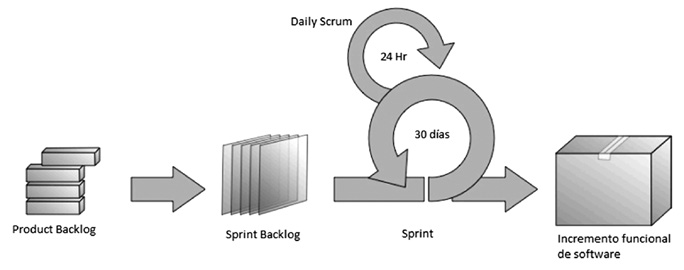
\includegraphics[width=11cm]{figuras/fasesDeUnSprint.png}}
    \caption{Ciclo de vida de un sprint}
    \label{fig::cicloDeVidaSprint}
\end{figure}

\begin{enumerate}
		\item \textbf{Planificación de la iteración (\textit{Sprint planning})}: se define el plan de trabajo de este Sprint especifico determinando qué se entregara y cómo se logrará. Es decir, se determinan las funcionalidades a implementar y la estimación de cantidad de trabajo. Con todo esto, y partiendo de la información en el \emph{Product backlog}, se establece el \emph{Sprint backlog}.
		\item \textbf{Reunión diaria (\textit{Daily meeting})}: cada día se realiza una reunión para explicar los objetivos que se han alcanzado desde la ultima reunión y determinar qué se realizará el día siguiente. Esto permite identificar problemas rápidamente y evitar que se retrase el ritmo de trabajo. \item \textbf{Revisión de la iteración (\emph{Sprint review})}: se realiza tras la finalización del Sprint completo. Se revisa todo lo que se hizo y lo que no, se comentan los problemas que tuvieron lugar y cómo se resolvieron, y se revisan los resultados obtenidos. 
		\item \textbf{Retrospectiva de la iteración (\emph{Sprint retrospective})}: esta reunión tiene el objetivo de analizar los puntos a mejorar y los puntos fuertes del equipo con el fin de aumentar la productividad.
		\item \textbf{Replanificación}: conjuntamente con el cliente se revisa la planificación teniendo en cuenta los posibles cambios que hayan podido surgir durante el \emph{Sprint}.
\end{enumerate}
			
\subsection{Aplicación de Scrum a este proyecto}
Dado que la mayoría de las practicas de Scrum están centradas en mejorar la productividad de un equipo, se han realizado una serie de adaptaciones teniendo en cuenta las características y circunstancias del proyecto. Se ha prescindido de la reunión diaria, pues el equipo de desarrollo está formado por una única persona. En este caso los sprints tuvieron una duración de inicial de 3 semanas, por lo que en lugar del \textit{Daily meeting} se ha optado por realizar una reunión semanal en la que se comentaba todo lo realizado hasta el momento y todas las actividades pendientes de abordar. Además, la reunión al final de cada sprint se realizó, en su mayoría, únicamente con los tutores y no con el cliente. Sin embargo, se mantuvo comunicación con este constantemente a lo largo de todo el desarrollo.

\subsection{DevOps}

Las antiguas metodologías de desarrollo de software separaban en dos sectores bien diferenciados aquellos que escribían el software (Dpto. Desarrollo) de aquellos que desplegaban en la nube (Dpto. Sistemas) \cite{devops5}.

DevOps surge con la idea de romper esta división y unir en un solo equipo a aquellos que desarrollan software y aquellos que lo despliegan. Esta unión proporciona transparencia a la hora de consultar el estado del producto y las distintas etapas que ha superado o superará.

La filosofía DevOps se basa en los mismos principios que las metodologías ágiles. Sin embargo, con DevOps se quiere fomentar una cultura de equipo, en la que todas las personas que formen el equipo sepan qué está haciendo cada una.

\subsubsection{Características de DevOps}
Esta filosofía busca la calidad de un producto software, creado por un equipo que se adapte rápido a los cambios e inconvenientes que aparezcan a lo largo de su desarrollo. Estos cambios deben ser identificados con rapidez para su posterior solución.

DevOps engloba todas las buenas prácticas a tener en cuenta a la hora de la entrega, el desarrollo y la administración de aplicaciones a lo largo del ciclo de vida de desarrollo de software: \cite{devops7}

\begin{itemize}
    \item Desarrollo y revisión de código con la ayuda de un controlador de versiones.
    \item Uso de herramientas de integración continua
    \item Continuo testeo del producto para obtener un software de calidad
    \item Uso de un gestor de repositorio optimizar la descarga y el almacenamiento de archivos binarios utilizados y producidos en el desarrollo de software.
    \item Uso de un gestor que automatice el proceso de despliegue
    \item Uso de un gestor de aprovisionamiento que nos cargue las configuraciones que necesarias de nuestro proyecto
    \item Monitorización del rendimiento de la aplicación
\end{itemize}

\subsection{Aplicación de DevOps a este proyecto}

Para este proyecto se usará Git \footnote{https://git-scm.com/} como herramienta para el control de versiones y GitHub \footnote{https://github.com/} como servicio público donde almacenar el repositorio de la aplicación.

Es fundamental en este proyecto el desarrollo basado en pruebas y la integración continua en el respositorio. El código debe de estar testeado previamente antes de añadirlo oficialmente al repositorio del mismo si se quiere obtener un software de calidad.

En este proyeco el equipo está formado por una persona, por lo que el mismo equipo será transparente y formado por el sector de desarrollo y el sector de despliegue.


\subsection{Combinación de Scrum y DevOps}

Como se ha explicado anteriormente, Scrum nos define un marco para el desarrollo de la aplicación. Un marco donde se definen Sprints para la consecución de objetivos.

Scrum se usará en este proyecto como una estructura que ayude a 

Dentro de cada Sprint, DevOps ayudará a la obtención de esos objetivos gracias a su filosofía, sobre todo su buena práctica relacionada en el desarrollo basado en pruebas, herramientas de automatización para el despliegue y la revisión del código gracias a un controlador de versiones.

\section{Gestión de la configuración}
En esta sección se define la gestión de la configuración bajo la cual desarrollaremos todas las actividades que impliquen la creación, modificación o eliminación de alguno de los elementos de trabajo que conforman este proyecto, asegurando así que todo lo que concierne al proyecto sea válido durante la vida del mismo.

 Teniendo en cuenta que los elementos de trabajo de este proyecto son los ficheros de código fuente y todos los archivos que conforman la documentación, abordaremos esta sección especificando, de forma independiente, cómo se ha tratado cada tipo de elemento de trabajo.
 
\subsection{Gestión del código}

Para la gestión del código se creará un repositorio local con un  sistema de control de versiones, que a su vez se sincronizará con un repositorio remoto en \textit{GitHub}, y por lo tanto almacenado en la nube. \textit{GitHub} es un servicio web de control de versiones y desarrollo de software basado en \textit{Git}, publicado bajo una Licencia de código abierto. Esta copia remota previene el riesgo de pérdida del código fuente.

\subsection{Gestión de la documentación}
Para almacenar la documentación de este proyecto se utilizará un repositorio en \textit{GitHub} llamado \textbf{Memoria\_TFG\_GuillermoMuriel} \footnote{https://github.com/guillesiesta/Memoria\_TFG\_GuillermoMuriel}.

Esta plataforma permite la creación de un repositorio cuyo lenguaje principal será LateX, y le añade una licencia de código abierto.

En cuanto a la edición y gestión de la memoria del proyecto, se utilizará la plataforma online \textit{Overleaf v2}\footnote{https://v2.overleaf.com/}. Dispone de control de versiones y edición en concurrencia. De la misma forma, al estar almacenada en la nube, se previene el riesgo de pérdida.

\section{Gestión del tiempo}
En este apartado se trata la planificación temporal del proyecto y las fases de la misma. Si bien se ha  establecido una planificación inicial, las tareas a realizar se especificarán de forma concreta a medida que se avance en el desarrollo del proyecto en función de los resultados obtenidos tras la finalización de cada sprint.

\subsection{Planificación de los sprints}

Teniendo en cuenta la metodología de desarrollo elegida, se ha optado por describir las tareas abordadas en cada sprint y su correspondiente gráfico \textit{Burn-Down}. Los diagramas \textit{Burn-down} son gráficos de dos ejes que se utilizan para representar el avance ideal del proyecto frente al avance real. En el eje X se representa el tiempo y en el eje Y la cantidad de trabajo. Es necesario actualizarlo diariamente. Antes, procederemos a introducir una visión general de los requisitos temporales escogidos sobre la organización del tiempo:

Disponemos de 300 horas para la realización del proyecto.

Para la realización de este proyecto se van a programar 5 sprints de 60 horas de duración cada uno. Por semana se trabajará de lunes a viernes unas 4 horas al día, en total 20 horas a la semana.

En total, se espera que cada sprint dure 3 semanas .

Por lo que el proyecto, salvo imprevisto, debería estar finalizado en torno a las 15 semanas. 

Aproximadamente debería concluir en 4 meses.

\begin{figure}[hbtp]
\begin{subfigure}{.5\textwidth}
    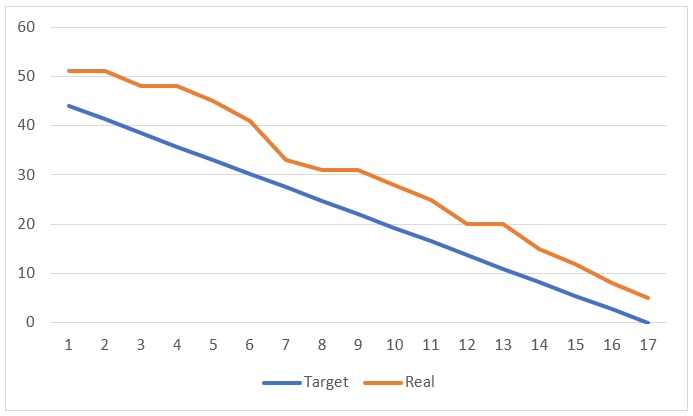
\includegraphics[width=\linewidth]{figuras/sprint1.png}
    \caption{Sprint 1}
    \label{fig:sprint1}
\end{subfigure}
\begin{subfigure}{.5\textwidth}
    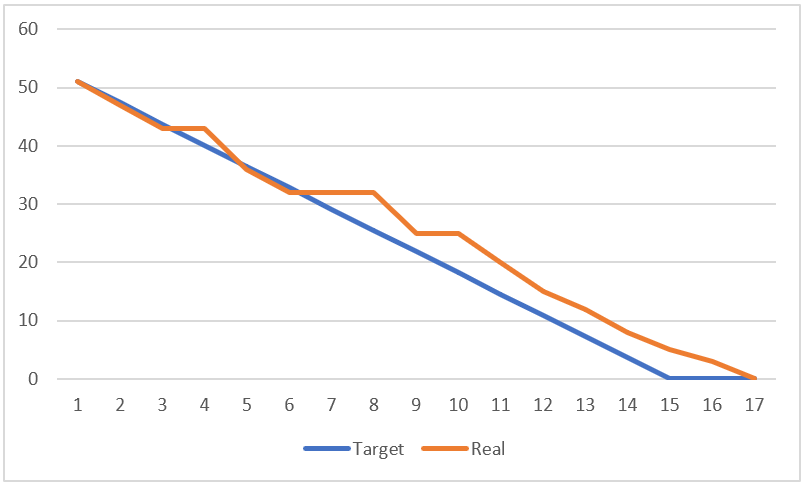
\includegraphics[width=\linewidth]{figuras/sprint2.png}
    \caption{Sprint 2}
    \label{fig:sprint2}
\end{subfigure}
\begin{subfigure}{.5\textwidth}
    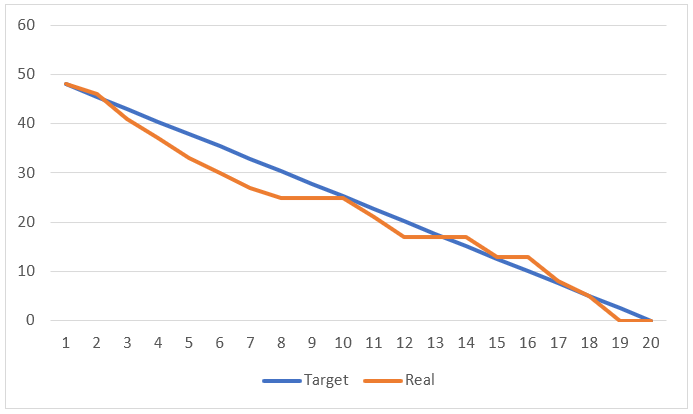
\includegraphics[width=\linewidth]{figuras/sprint3.png}
    \caption{Sprint 3}
    \label{fig:sprint3}
\end{subfigure}
\begin{subfigure}{.5\textwidth}
    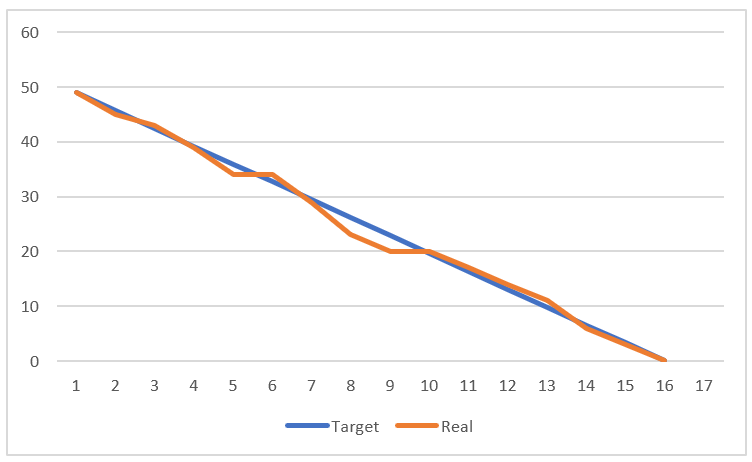
\includegraphics[width=\linewidth]{figuras/sprint4.png}
    \caption{Sprint 4}
    \label{fig:sprint4}
\end{subfigure}
\begin{subfigure}{\textwidth}
    \centering
    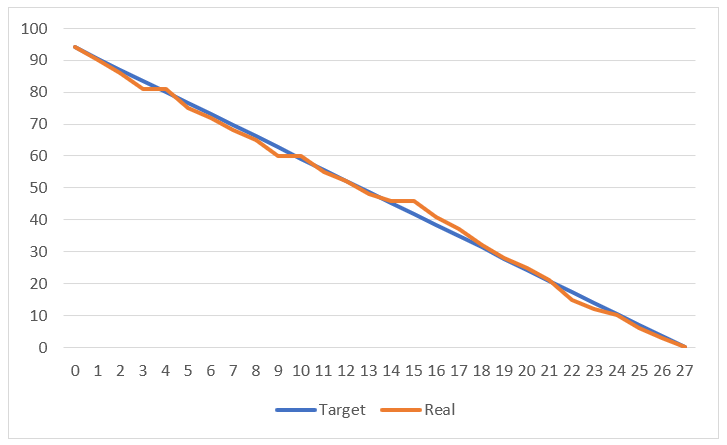
\includegraphics[width=.5\linewidth]{figuras/sprint5.png}
    \caption{Sprint 5}
    \label{fig:sprint5}
\end{subfigure}
\caption{Gráficos \textit{burn-down} de los distintos sprints del proyecto}
\label{fig:sprints}
\end{figure}

\begin{itemize}
    \item \textbf{Sprint 1}. En esta primera fase determinará la organización temporal y se estudiará la viabilidad del proyecto. Se extraerán los requisitos y a partir de estos se hará un análisis de las tecnologías existentes para poder desarrollar nuestro proyecto y desplegarlo en la nube y, se escogerán cuales serán las herramientas que más se adecúen a las necesidades del proyecto.
    
    \item \textbf{Sprint 2}. En esta segunda fase se comenzará a trabajar en el almacenamiento de datos, se extraerá toda la documentación necesaria y se procederá a la construcción de la misma. Nuestra base de datos debe estar organizada, estructurada y desarrollada para que en el siguiente sprint ya pueda ser utilizada.
    \item \textbf{Sprint 3}. En este sprint se procederá a construir nuestro intermediario entre la interfaz y la base de datos. Lo llamaremos controlador, es decir, nuestra API REST. Además, se implementaran tests que este controlador deberá de superar, así se confirma su correcto funcionamiento antes del montaje final. En esta fase conectaremos nuestro controlador a nuestra base de datos.
    \item \textbf{Sprint 4}. Esta fase está desarrollada única y enteramente al desarrollo de nuestra interfaz. Se escribirán los tests que deben de ser superados para que nuestra interfaz sea apta para su despliegue.
    \item \textbf{Sprint 5}. En la fase final se procederá a la unión de nuestra interfaz y nuestro controlador ya unido con la base de datos. A partir de aquí, con nuestro sistema funcionando y testeado, procederemos a desplegarlo usando las tecnologías escogidas previamente. 
    
    Una vez la aplicación esté desplegada, se procederá a la redacción de la memoria.
\end{itemize}

\section{Gestión de riesgos}
Un riesgo de un proyecto es un evento o condición  que podría tener un efecto positivo o negativo sobre alguno de los recursos u objetivos del proyecto, como podría ser tiempo, coste, alcance o calidad. La gestión de riesgos es un proceso continuo que debe considerar tanto fuentes internas como externas de dichos riesgos. Por norma general, la materialización de un riesgo implica consecuencias negativas, por lo que la gestión de riesgos tiene un papel muy importante dentro de la gestión del proyecto. 

En esta sección se identificarán los posibles riesgos del proyecto, estimando la probabilidad de aparición y su impacto potencial. Posteriormente se definirán las estrategias y pasos a seguir para prevenirlos o minimizar su impacto en caso de que se materialicen.

\subsection{Identificación de riesgos}
\begin{itemize}
\item \textbf{R001} - No identificar correctamente los requisitos del proyecto.
\item \textbf{R002} - Dificultad en las tareas de formación.
\item \textbf{R003} - Aparición de nuevos requisitos.
\item \textbf{R004} - No conseguir ajustar la planificación a las horas requeridas.
\item \textbf{R005} - Cambios en la planificación o retrasos en la misma.
\item \textbf{R006} - Errores eligiendo las tecnologías para el desarrollo del proyecto.
\item \textbf{R007} - Disponibilidad del experto insuficiente.
\item \textbf{R008} - La estructura de los datos de partida cambia con el tiempo.
\item \textbf{R009} - Nulo o deficiente proceso de validación y verificación .
\item \textbf{R010} - Detección de fallos importantes en el software tras la validación.
\item \textbf{R011} - Detección de fallos importantes en los resultados tras la validación.
\item \textbf{R012} - La interfaz no cumple con los requisitos.
\item \textbf{R013} - La API no cumple con los requisitos.
\item \textbf{R014} - La base de datos escogida no cumple con los requisitos.
\item \textbf{R015} - Pérdida de parte del proyecto (documentación o código).
\item \textbf{R016} - Computador de desarrollo estropeado.
\item \textbf{R017} - Se sobrepasan los límites de los servicios gratuitos de las plataformas escogidas.
\item \textbf{R018} - La plataforma GitHub no está disponible.
\item \textbf{R019} - Las tecnologías usadas cambian de versión durante el proceso de desarrollo.
\item \textbf{R020} - Problemas de transporte de información entre las tecnologías implementadas.
\end{itemize}

\subsection{Planificación de la respuesta a los riesgos}
\subsection{Riesgos materializados}

\section{Gestión de costes}
\subsection{Costes de recursos humanos}
\subsection{Costes de material}
\subsection{Costes de indirectos}
\subsection{Costes total del proyecto}



\chapter{Especificación de Requisitos}
Los requisitos se pueden definir como aquellas características esperables y/o deseables que debe cumplir un sistema para satisfacer unas necesidades especificas. Esta tarea es imprescindible para asegurar el éxito del proyecto. En esta sección describiremos los requisitos del proyecto desde una perspectiva menos tradicional que encaja mejor con la metodología de desarrollo elegida: historias de usuario. Las historias de usuario describen de forma breve aquello que un determinado usuario (en este caso desarrollador) espera al final del desarrollo. Es necesario que cumplan una serie de características:
\begin{itemize}
    \item Deben ser independientes.
    \item Ser negociables. No actúan como un contrato, sino como una serie de pautas de acción.
    \item Deben aportar valor al proyecto.
    \item Se debe poder realizar una estimación sobre ellas (temporal o de carga de trabajo).
    \item Deben tener un tamaño manejable.
    \item Deben ser verificables, pues es necesario saber si una historia se ha cumplido.
\end{itemize}

Cada historia se ha expresado siguiendo el siguiente patrón:
\begin{center}
    Como \texttt{<usuario>}, quiero / espero \texttt{<objetivo>}
\end{center}

Además cada una de ellas se acompaña de una estimación temporal, unos criterios de aceptación, un nivel de importancia y un identificador.

Se distinguirán entre tres tipos de niveles de importancia, según su prioridad.
\begin{itemize}
    \item \textbf{Alta} (Cumplimiento obligatorio): la historia es imprescindible para el desarrollo y éxito del proyecto. Es necesario que esté en la versión final para aceptar el proyecto.
    \item \textbf{Media} (Cumplimiento deseable): es deseable la presencia de esta historia en la versión final del proyecto, pero no supone un aumento significativo del valor del producto.
    \item \textbf{Baja} (Cumplimiento opcional): su presencia no es crucial para el éxito del proyecto, pero aporta cierto valor funcional. 
\end{itemize}

Aún cuando el tiempo total de todas las historias de usuario sea mayor al tiempo disponible, no supone un inconveniente, pues las historias se desarrollarán más de una a la vez ya que se solapan y es casi imposible determinar tareas aisladas para el cumplimiento de cada una.

A continuación se especificarán todas las historias de usuario del proyecto teniendo en cuenta el  documento guía \ref{tab:HC-EJEMPLO} para la especificación de historias de usuario.

\begin{table}[htbp]
\centering
\begin{tabular}{|c|L{10.5cm}|}
    \hline
    \multicolumn{2}{|l|}{\textbf{Código} - Nombre} \\\hline 
    \textbf{Descripción}	&  Breve descripción de la historia de usuario. \\\hline
    \textbf{Estimación}	&	Estimación temporal de la historia. 	\\\hline
    \textbf{Prioridad}	&	Prioridad según la importancia que tiene esta historia para el desarrollo satisfactorio del proyecto.	\\\hline
    \textbf{Aceptación}	&	Criterios a cumplir para considerar que esta historia de usuario se ha cubierto satisfactoriamente.		\\\hline
    \textbf{Notas}		&	Observaciones varias.		\\\hline
\end{tabular}
\caption{Documento guía. Especificación de las historias de usuario.}
\label{tab:HC-EJEMPLO}
\end{table}

\section{Historias de usuario}

\begin{table}[H]
\centering
\label{tab:HU-0}
\begin{tabular}{|c|L{10.5cm}|}
    \hline
    \multicolumn{2}{|l|}{\textbf{HU-00} -Proponer una solución a un acertijo} \\\hline 	
    \textbf{Descripción}	& Quiero que el usuario sea capaz de proponer soluciones a los acertijos del sistema
	\\\hline
    \textbf{Estimación}	&	3 semanas	\\\hline
    \textbf{Prioridad}	&	Alta		\\\hline
    \textbf{Aceptación}	&	En el caso de que el usuario introduzca correctamente una solución a un acertijo, ésta se almacenará en la plataforma y se enlazará con el acertijo	\\\hline
    \textbf{Notas}		&			\\\hline
\end{tabular}
\end{table}

\begin{table}[H]
\centering
\label{tab:HU-1}
\begin{tabular}{|c|L{10.5cm}|}
    \hline
    \multicolumn{2}{|l|}{\textbf{HU-01} - Login o acceso a la aplicación} \\\hline 	
    \textbf{Descripción}	& Quiero que el usuario acceda a la plataforma a través de usuario y contraseña
	\\\hline
    \textbf{Estimación}	&	3 semanas	\\\hline
    \textbf{Prioridad}	&	Alta		\\\hline
    \textbf{Aceptación}	&	En el caso de que el usuario introduzca correctamente su usuario y contraseña, se accederá a la plataforma	\\\hline
    \textbf{Notas}		&			\\\hline
\end{tabular}
\end{table}

\begin{table}[H]
\centering
\label{tab:HU-2}
\begin{tabular}{|c|L{10.5cm}|}
    \hline
    \multicolumn{2}{|l|}{\textbf{HU-02} - Escribir un acertijo} \\\hline 	
    \textbf{Descripción}	& Quiero que el usuario sea capaz de escribir un acertijo y subirlo a la plataforma
	\\\hline
    \textbf{Estimación}	&	3 semanas	\\\hline
    \textbf{Prioridad}	&	Alta		\\\hline
    \textbf{Aceptación}	&	Cuando el usuario introduzca su acertijo, éste deberá ser accesible en la plataforma	\\\hline
    \textbf{Notas}		&			\\\hline
\end{tabular}
\end{table}

\begin{table}[H]
\centering
\label{tab:HU-3}
\begin{tabular}{|c|L{10.5cm}|}
    \hline
    \multicolumn{2}{|l|}{\textbf{HU-03} - Consulta de propios acertijos} \\\hline 	
    \textbf{Descripción}	& Quiero que el usuario sea capaz de consultar el estado de sus acertijos
	\\\hline
    \textbf{Estimación}	&	3 semanas	\\\hline
    \textbf{Prioridad}	&	Media		\\\hline
    \textbf{Aceptación}	&	Cuando el usuario introduzca su acertijo, éste deberá ser accesible en la plataforma en un apartado en que solamente se muestren los acertijos escritos del usuario	\\\hline
    \textbf{Notas}		&			\\\hline
\end{tabular}
\end{table}

\begin{table}[H]
\centering
\label{tab:HU-4}
\begin{tabular}{|c|L{10.5cm}|}
    \hline
    \multicolumn{2}{|l|}{\textbf{HU-04} - Puntuación de las respuestas de un acertijo} \\\hline 	
    \textbf{Descripción}	& Quiero que el usuario sea capaz de puntuar las respuestas propuestas por los demás usuarios sobre sus acertijos
	\\\hline
    \textbf{Estimación}	&	3 semanas	\\\hline
    \textbf{Prioridad}	&	Alta		\\\hline
    \textbf{Aceptación}	&	Cuando el usuario acceda a las soluciones del acertijo y modifique la puntuación de la solución, ésta deberá ser actualizada al momento.	\\\hline
    \textbf{Notas}		&			\\\hline
\end{tabular}
\end{table}

\begin{table}[H]
\centering
\label{tab:HU-5}
\begin{tabular}{|c|L{10.5cm}|}
    \hline
    \multicolumn{2}{|l|}{\textbf{HU-05} - Actualización del porcentaje del estado de un acertijo } \\\hline 	
    \textbf{Descripción}	& Quiero que sistema actualice el estado de un acertijo basándose en las puntuaciones obtenidas de las respuestas propuestas al mismo
	\\\hline
    \textbf{Estimación}	&	3 semanas	\\\hline
    \textbf{Prioridad}	&	Alta		\\\hline
    \textbf{Aceptación}	&	Cuando el usuario acceda a un acertijo, éste mostrará el estado de resolución en el que se encuentra	\\\hline
    \textbf{Notas}		&			\\\hline
\end{tabular}
\end{table}

\begin{table}[H]
\centering
\label{tab:HU-6}
\begin{tabular}{|c|L{10.5cm}|}
    \hline
    \multicolumn{2}{|l|}{\textbf{HU-06} - Consulta de todas las soluciones propuestas a un acertijo } \\\hline 	
    \textbf{Descripción}	& Quiero que un usuario al acceder a un acertijo a resolver, tenga la posibilidad de consultar todas las propuestas como solución escritas para el mismo
	\\\hline
    \textbf{Estimación}	&	3 semanas	\\\hline
    \textbf{Prioridad}	&	Alta		\\\hline
    \textbf{Aceptación}	&	Al acceder a un acertijo, si éste tiene soluciones, deberán mostrarse en el caso de que el usuario lo solicite 	\\\hline
    \textbf{Notas}		&			\\\hline
\end{tabular}
\end{table}

\begin{table}[H]
\centering
\label{tab:HU-7}
\begin{tabular}{|c|L{10.5cm}|}
    \hline
    \multicolumn{2}{|l|}{\textbf{HU-07} -Modificación de los datos de un usuario } \\\hline 	
    \textbf{Descripción}	& Quiero que un usuario pueda modificar sus datos
	\\\hline
    \textbf{Estimación}	&	3 semanas	\\\hline
    \textbf{Prioridad}	&	Baja		\\\hline
    \textbf{Aceptación}	&	Al acceder a sus datos personales y modificarlos, éstos se actualizarán automáticamente en el sistema 	\\\hline
    \textbf{Notas}		&	Esta funcionalidad se contemplará única y exclusivamente cuando se disponga de tiempo de más en el sprint correspondiente		\\\hline
\end{tabular}
\end{table}


\begin{table}[H]
\centering
\label{tab:HU-8}
\begin{tabular}{|c|L{10.5cm}|}
    \hline
    \multicolumn{2}{|l|}{\textbf{HU-08} - Adaptabilidad a distintos front-ends } \\\hline 	
    \textbf{Descripción}	& Quiero que mi aplicación sea adaptable a distintos front-end
	\\\hline
    \textbf{Estimación}	&	3 semanas	\\\hline
    \textbf{Prioridad}	&	Alta		\\\hline
    \textbf{Aceptación}	&	La API desarrollada debe de ser accesible desde cualquier lugar y en cualquier momento. Esto es, debe permitir el acceso a peticiones HTTP. 	\\\hline
    \textbf{Notas}		&			\\\hline
\end{tabular}
\end{table}

\begin{table}[H]
\centering
\label{tab:HU-10}
\begin{tabular}{|c|L{10.5cm}|}
    \hline
    \multicolumn{2}{|l|}{\textbf{HU-10} - Interfaz sencilla e intuitiva } \\\hline 	
    \textbf{Descripción}	& Quiero que mi aplicación sea fácil de usar y atractiva
	\\\hline
    \textbf{Estimación}	&	3 semanas	\\\hline
    \textbf{Prioridad}	&	Alta		\\\hline
    \textbf{Aceptación}	&	La interfaz no contendrá excesiva carga de información, y será intuitiva 	\\\hline
    \textbf{Notas}		&			\\\hline
\end{tabular}
\end{table}

\begin{table}[H]
\centering
\label{tab:HU-11}
\begin{tabular}{|c|L{10.5cm}|}
    \hline
    \multicolumn{2}{|l|}{\textbf{HU-11} - Accesibilidad y gestión de los datos } \\\hline 	
    \textbf{Descripción}	& Quiero que la base de datos de mi aplicación sea sencilla de administrar y que acepte peticiones HTTP de mi API
	\\\hline
    \textbf{Estimación}	&	3 semanas	\\\hline
    \textbf{Prioridad}	&	Alta		\\\hline
    \textbf{Aceptación}	&	La base de datos no dispondrá de excesiva complejidad y será accesible, alojándose ésta en la nube 	\\\hline
    \textbf{Notas}		&			\\\hline
\end{tabular}
\end{table}

\begin{table}[H]
\centering
\label{tab:HU-12}
\begin{tabular}{|c|L{10.5cm}|}
    \hline
    \multicolumn{2}{|l|}{\textbf{HU-12} - Tecnologías usadas libres } \\\hline 	
    \textbf{Descripción}	& Quiero desarrollar mi aplicación con software libre
	\\\hline
    \textbf{Estimación}	&	3 semanas	\\\hline
    \textbf{Prioridad}	&	Media		\\\hline
    \textbf{Aceptación}	&	La mayor parte de la aplicación deberá estar desarrollada con software libre 	\\\hline
    \textbf{Notas}		&			\\\hline
\end{tabular}
\end{table}

\chapter{Análisis}
En este capítulo se aborda la fase de análisis de los distintos requerimientos  del sistema para cumplir con los objetivos del proyecto. 
La tarea principal será cumplir estos requerimientos de la manera más eficaz posible.
\section{Requisitos de la aplicación}
\section{Tecnologías a emplear}

\chapter{Diseño}

\section{Arquitectura}
\subsection{Arquitectura Cliente-Servidor}

\section{Diseño}
\subsection{Representación de los datos}
\subsection{Determinación del contenido}
\subsection{Módulo de gestión conversacional}
\subsection{Paquetes}

\chapter{Implementación y funcionamiento del sistema}


\chapter{Pruebas}

\chapter{Conclusiones}

\begin{thebibliography}{999}

\bibitem{licenciaproyecto} 
GNU General Public License v3.0,
\\\texttt{https://github.com/guillesiesta/ProjectX/blob/master/LICENSE}

\bibitem{nube1} 
Computación en la nube, Wikipedia
\\\texttt{https://es.wikipedia.org/wiki/Computación\_en\_la\_nube}

\bibitem{frontback} 
Computación en la nube, Wikipedia
\\\texttt{https://es.wikipedia.org/wiki/Front-end\_y\_back-end}

\bibitem{api1} 
¿Qué es una API REST?, Jonathan Ordóñez
\\\texttt{https://www.idento.es/blog/desarrollo-web/que-es-una-api-rest/}

\bibitem{api2} 
Relationship to the World Wide Web and REST Architectures, W3C Working Group Note 11 February 2004
\\\texttt{https://www.w3.org/TR/2004/NOTE-ws-arch-20040211/\#relwwwrest}

\bibitem{api3} 
CHAPTER 5, Representational State Transfer (REST)
\\\texttt{https://www.ics.uci.edu/~fielding/pubs/dissertation/rest\_arch\_style.htm}

\bibitem{devops1} 
DevOps Culture (Part 1), May 1, 2012 by John Willis,
\\\texttt{http://itrevolution.com/devops-culture-part-1/}

\bibitem{devops2}
The Rise of DevOps, 02 Mar 2010, Dmitriy Samovskiy's Blog,
\\\texttt{http://www.somic.org/2010/03/02/the-rise-of-devops/}

\bibitem{devops3} 
What is DevOps?,by Mike Loukides, June 7, 2012
\\\texttt{http://radar.oreilly.com/2012/06/what-is-devops.html}

\bibitem{devops4} 
Desarrollo basado en pruebas, Material docente para Infraestructura Virtual, Juan Julián Merelo Guervós
\\\texttt{http://jj.github.io/IV/documentos/temas/Desarrollo\_basado\_en\_pruebas\
\#gestores-de-versiones-de-lenguajes-y-bibliotecas}

\bibitem{devops5} 
DevOps: cómo romper la barrera entre Desarrollo y Operaciones, Atlassian
\\\texttt{https://es.atlassian.com/devops}

\bibitem{devops6} 
 Vayamos al grano, ¿qué es eso de DevOps?,  Ana M. del Carmen García Oterino
\\\texttt{http://www.javiergarzas.com/2014/12/devops-en-10-min.html}

\bibitem{devops7} 
 Exploring the ENTIRE DevOps Toolchain for (Cloud) Teams,  Richard Seroter on May 28, 2014
\\\texttt{https://www.infoq.com/articles/devops-toolchain}

\bibitem{proyectogithub} 
Project X , Guillesiesta,
\\\texttt{https://github.com/guillesiesta/ProjectX}

\bibitem{desarrollotests} 
The Relationship Between Dev-Ops And Continuous Delivery: A Conversation With Jez Humble Of ThoughtWorks , Jeffrey Hammond,
\\\texttt{https://go.forrester.com/blogs/11-09-09-the\_relationship
\_between\_dev\_ops\_and\_continuous\_delivery\_a\_conversation\_
with\_jez\_humble\_of\_thought/}

\bibitem{desarrollotests2} 
Continuous delivery, wikipedia
\\\texttt{https://en.wikipedia.org/wiki/Continuous\_delivery}

\bibitem{cors} 
Control de acceso HTTP (CORS), MDN Dev Docs
\\\texttt{https://developer.mozilla.org/es/docs/Web/HTTP/Access\_control\_CORS}


\bibitem{corsflask} 
Python Flask Cors Issue ,stackoverflow
\\\texttt{https://stackoverflow.com/questions/28461001/python-flask-cors-issue}

\bibitem{corsflask2} 
Flask-CORS
\\\texttt{https://flask-cors.readthedocs.io/en/latest/}

\bibitem{guiahays} 
Guía Hays del mercado laboral 2018
\\\texttt{http://guiasalarial.hays.es/trabajador/info-sector}

\bibitem{costeindirecto} 
Coste Indirecto Proyecto UGR
\\\texttt{http://investigacion.ugr.es/pages/proyectosja/2018/ayuda}


\bibitem{mvc1} 
Modelo–vista–controlador, Wikipedia
\\\texttt{https://es.wikipedia.org/wiki/Modelo-Vista-Controlador}

\bibitem{mvc2} 
Simple Example of MVC (Model View Controller), Design Pattern for Abstraction
\\\texttt{https://www.codeproject.com/Articles/25057/
Simple-Example-of-MVC-Model-View-Controller-Design}

\bibitem{mvc3} 
Applications Programming in Smalltalk-80(TM):
How to use Model-View-Controller (MVC), by Steve Burbeck
\\\texttt{https://web.archive.org/web/20120429161935/
http://st-www.cs.illinois.edu/users/smarch/st-docs/mvc.html}


\bibitem{tipobd} 
Bases de datos ¿qué son? ¿qué tipos existen? Lo que necesitas saber como profesional, Maldeadora
\\\texttt{https://platzi.com/blog/bases-de-datos-que-son-que-tipos-existen/}

\bibitem{tipobd2} 
Tipos de bases de datos no relacionales, Wikipedia
\\\texttt{https://es.wikipedia.org/wiki/NoSQL}

\bibitem{bdnorel1} 
Global Graph Database Market is Expected to To Reach Around USD 5.6 Billion by 2024, Allan , Sep 3, 2018
\\\texttt{https://zmrnewsjournal.us/1265/global-graph-
database-market-is-expected-to-to-reach-around-usd-5-6
-billion-by-2024/}


\bibitem{bdnorel2} 
Global Graph Database Market 2018 – 2025 triAGENS GmbH(Arango DB), Neo4j, Inc, OrientDB Ltd, Cayley, Titan, MarkLogic, johnsgaston, September 5, 2018 
\\\texttt{http://lakeviewgazette.com/2018/09/05/global-graph
-database-market-2018-2025-triagens-gmbharango-db-neo4j-inc
-orientdb-ltd-cayley-titan-marklogic/}

\bibitem{neovstitan} 
anybody tried neo4j vs titan - pros and cons [closed], StackOverflow
\\\texttt{https://stackoverflow.com/questions/17269306/anybody-tried-neo4j-vs-titan-pros-and-cons}

\bibitem{apirest1} 
What are the best programming languages for building APIs? , Antonio Cucciniello , June 11, 2017
\\\texttt{https://hub.packtpub.com/what-are-best-programming-languages-building-apis/}

\bibitem{apirest2} 
What Languages Should Your API Helper Libraries Support?,  Bill Doerrfeld November 12,2015
\\\texttt{https://nordicapis.com/what-languages-
should-your-api-helper-libraries-support/}

\bibitem{apirest3} 
What Languages Should Your API Helper Libraries Support?,  Bill Doerrfeld November 12,2015
\\\texttt{https://nordicapis.com/what-languages-
should-your-api-helper-libraries-support/}

\bibitem{flaskvsdjango1} 
Flask vs Django, Scott Robinson, September 21, 2017
\\\texttt{https://stackabuse.com/flask-vs-django/}

\bibitem{framework} 
Los 5 mejores frameworks de JavaScript en 2017, CampusMVP
\\\texttt{https://www.campusmvp.es/recursos/post/los-5-mejores-frameworks-de-javascript-en-2017.aspx}

\bibitem{framework2} 
JavaScript Framework Guide AND Top 15 JS Frameworks of 2019 Prediction, Gurdeep Singh, Friday, June 15, 2018
\\\texttt{https://appinventiv.com/blog/javascript-framework-guide}

\bibitem{cloud} 
¿Cuál es la diferencia entre IaaS, SaaS y PaaS?, Scott Carey 
\\\texttt{http://www.ciospain.es/gobierno-ti/
cual-es-la-diferencia-entre-iaas-saas-y-paas}

\bibitem{cloud2} 
Cloud Computing, Wikipedia
\\\texttt{https://en.wikipedia.org/wiki/Cloud\_computing}

\bibitem{cloud3} 
IaaS, PaaS y SaaS, ¿cuáles son sus diferencias?, Angel Carrero, 22 julio, 2016 
\\\texttt{https://revistacloud.com/iaas-paas-y-saas-cuales-son-sus-diferencias/}

\bibitem{cloud4} 
Servicios en la nube: diferencias entre IaaS, SaaS y PaaS,  T. Mora on 2 noviembre 2017 
\\\texttt{http://blog.neteris.com/stepforward/servicios-en-la-nube-diferencias-entre-iaas-saas-y-paas}

\bibitem{clienteservidor} 
Cliente Server, Wikipedia
\\\texttt{https://en.wikipedia.org/wiki/Client\_server\_model}


\end{thebibliography}



%%\chapter{Conclusiones y Trabajos Futuros}

\nocite{*}
\bibliography{capitulos/bibliografia}\addcontentsline{toc}{chapter}{Bibliografía}
\bibliographystyle{miunsrturl}

%\appendix
%\input{apendices/manual_usuario/manual_usuario}
%%\input{apendices/paper/paper}
%\input{glosario/entradas_glosario}
% \addcontentsline{toc}{chapter}{Glosario}
% \printglossary
\chapter*{}
\thispagestyle{empty}

\end{document}
